
\subsubsection{Idea}

To compute the serie of $(x+1)^{2^i}$, we have different ways to proceed. But all the classic ways are not necessary the best to compute all the coefficients. \\

If we need all the $(x+1)^j$ for $j \in \mbox{\textlbrackdbl} 1, n\mbox{\textrbrackdbl}$, it will be better to use the formula ${n+1 \choose k+1} = {n \choose k} + {n \choose k+1}$ to compute each element and proceed to a divide and conquer method to compute in parallel the coefficients. But, we just need the coefficients of $(x+1)^{2^i}$. Then, if we proceed with a divide and conquer on all the elements of $(x+1)^j$ and just keep the $(x+1)^{2^i}$, we can have a lot of computations, in particular for $i$ big, which won't be stored and just be needed to go to the next power of $(x+1)$. That's not what we want, so we will use the formula of the binomial coefficients with the factorial sequence to get directly the coefficient of each $(x+1)^{2^i}$. \\

With the method I will explain in this part, I think we loose a little time at the beginning, computing yet the factorial sequence in parallel. But after, the computations are fast and nothing is superfluous.\\

So, to compute the Newton's binomial coefficients, we want to use the following formula :
$$\forall n\in \mathbb{N},\, (x+1)^n = \sum_{k=0}^{n} {n \choose k}\, x^k \mbox{ with } {n \choose k} = \cfrac{n!}{k!\, (n-k)!}$$

We need so to compute all the elements $i! \forall i\in \mbox{\textlbrackdbl} 0, n\mbox{\textrbrackdbl}$.

\subsubsection{The sequence of factorials}

To use the previous formula to get all the binomials' coefficients, we need the values of each $i! \mod p$ for $i \in \mbox{\textlbrackdbl} 0, n\mbox{\textrbrackdbl}$.

One may notice that to obtain $i!$, we need $(i-1)!$. So if we consider the computation in serie of all the $i!$, it may be very long to obtain $n!$ for $n$ big. \\

First of all, we need an array of size $n+1$, called \textit{Factorial\_device} in my code as we also need $0!$. But we don't really need to compute $0! = 1$ so we'll consider the following computations on \textit{Factorial\_device + 1} thus we just compute $i!$ for $i \in \mbox{\textlbrackdbl} 1, n\mbox{\textrbrackdbl}$. Now we consider computations of size $n = 2^e$ with $e \in \mathbb{N}^*$. As $n$ is a power of $2$, I was looking for a code to compute pairwise elements.

\subsubsection{Mapping for the computation of the factorial sequence}

To understand the code, see the following picture from the bottom which is the first step : the initialization. First we initialize the array \textit{Factorial\_device + 1} letting the even elements as their position and we do multiplications on the odd elements. \\

Then, in each step, we consider the array per parts. We can see a part in each step as the following : we multiply the element of a position by a same number for a part, these 'same numbers' are what I call "pillar factors", represented by the darkest boxes. We can see that step after step, we compute several $i!$ in parallel and finally get every $i!$ in $\log_{2}(n)$ steps.\\

\begin{center}
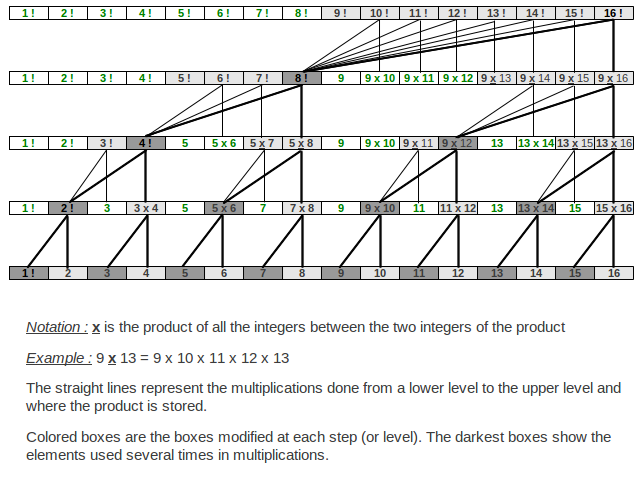
\includegraphics[scale=0.8]{facto.png}
\end{center}

See in the \textbf{Appendix} the file \textit{Taylor\_shift\_kernel.cu} and in particular the procedures \textit{identity\_GPU}, \textit{create\_factorial\_step0\_GPU} and \textit{create\_factorial\_stepi\_GPU} which correspond to the different steps of the computation in parallel of the sequence of factorials. First we inialise the $n+1$ positions in the array \textit{Factorial\_device} with their position or 1 for \textit{Factorial\_device[0]} with \textit{identity\_GPU} and then the two others procedure modified $n/2$ positions of the array at each step. The procedure \textit{create\_factorial\_stepi\_GPU} has only one problem, if we take a look at the previous graphic we can see that in each step, a lot of threads will need the same "pillar factor", so many threads will take the value of a same position in the array at the same time, there is an overlap reducing performances of the code. This part needs to be worked to find another way to do the computation of the factorial elements to improve a little more the efficiency of my code.

\subsubsection{The array of the $(x+1)^{2^i}$}
To do the Taylor shift by 1, we need to compute all the $(x+1)^{2^i}$ as we said before. As now we have the sequence of the factorials, we can compute in parallel each coefficient of the $(x+1)^{2^i}$  but do we we really need all of them ? \\

If we look at the following Pascal triangle until the binomial coefficients of $(x+1)^{8}$, naively we just need to use the coefficients colored in yellow. But, a lot of them are $1$, we can avoid to have too much ones in the array. Moreover, we don't really need $(x+1)^0$. We want also to store these coefficients in an array of $1$ dimension so successively. If we store the coefficients naively, we will store the following sequence : $1,1,1,1,2,1,1,4,6,4,1,1,8,28,56,70,56,28,8,1$. We have to keep in mind also that when we will need to use $(x+1)^{2^i}$, we will need to know the position of this $(x+1)^{2^i}$ in our array. \\

\begin{center}
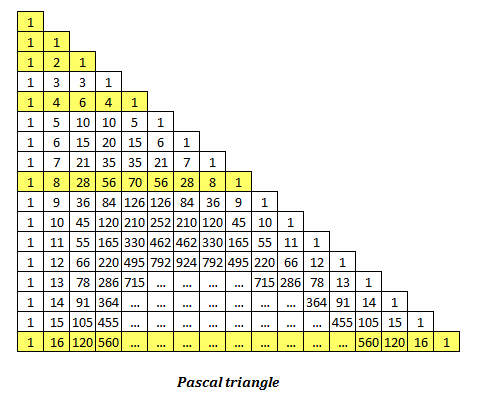
\includegraphics[scale=1]{PascalTriangle.png}
\end{center}

Now, if we avoid all the ones in the first column of the Pascal triangle (except the first for $(x+1)^0$, even though it is useless), the sequence to store becomes : $1,1,2,1,4,6,4,1,8,28,56,70,56,28,8,1$. This sequence is better as the coefficients of $(x+1)^{2^i}$ are easily found at the position $2^i-1$ (except for the first but keep in mind it is useless). Thus, most of the ones in this sequences can be used to represent two consecutives $(x+1)^{2^i}$.\\

Moreover, for a polynomial of degree $n$, this array is of size... $n$ ! So like this, this array will be very practical to use. For $n = 16 = 2^4$, we will use the following array :\\

\begin{center}
\begin{tabular}{|c||c||c|c||c|c|c|c||c|c|c|c|c|c|c|c||} \hline
1 & 1 & 2 & 1 & 4 & 6 & 4 & 1 & 8 & 28 & 56 & 70 & 56 & 28 & 8 & 1 \\ \hline
\end{tabular}
\end{center}

This array is called \textit{Monomial\_shift\_device} in the code and created by the procedure \textit{develop\_x\_shift}. Each thread need first of all to know what $(x+1)^{2^i}$ it deals with and after the coefficient it needs to compute with the function \textit{create\_binomial2\_GPU}.\\

One may notice that if we think more on how to reduce computations, the Pascal triangle is symmetric. So approximatively the half of the coefficients don't really need to be stored as I do for the moment. For example, in the case $n=16$ I have taken, we could just store $1,2,4,6,8,28,56,70$ which will be an array of size $n/2$ and after find a way to use this smaller array correctly to use the coefficient. It is possible and it is a way of reflection I keep in mind when we will try to improve our code when it will be completely finished.\\
